\documentclass[fr]{../../../../../../epltest}


\hypertitle{Compléments d'électricité (partie dispositifs)}{5}{ELEC}{1330}{2017}{Novembre}{All}
{Maxime Wattiaux \and Martin Braquet}
{Denis Flandre}

\section{Exercice (questionnaire A)}

On considère la jonction NP en silicium représentée sur la figure 1 ci-dessous. La zone N ainsi que la zone de déplétion sont protégées de toute illumination par un cache. La zone P n'est par contre pas couverte et est soumise à une génération linéaire $G(x)=G_1x+G_2$. La structure est suffisamment fine ($h \approx 0$) de sorte que les termes de génération peuvent être considérés constants selon la direction $y$. La zone de déplétion est supposée équitablement répartie entre les deux zones N et P, et est de longueur $d$ donnée. On supposera que la génération/recombinaison dans cette zone est négligeable. Une différence de potentiel $V$ est appliquée aux bornes de la diode (entre $x = - x_n$ et $x= x_p$) via des contacts ohmiques. On suppose $N_A$ et $N_D$ connus ainsi que $D_n$, $D_p$, $\tau_n$, $\tau_p$, $T$, $V$, $G_1$ et $G_2$.

On supposera également que $x_p$ >> $L_n$ et $x_n$ << $L_p$.

\begin{figure}[h!]
	\centering
	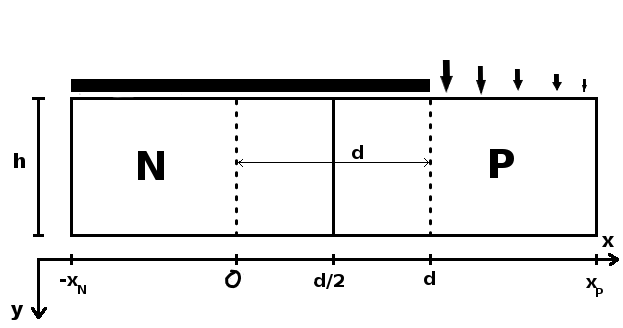
\includegraphics[scale=0.5]{interroA.png}
	\caption{Jonction NP}
	\label{Jonction NPA}
\end{figure}

On vous demande de trouver l'équation de la densité de courant $J$ dans la diode. \\

Énoncez et justifiez clairement toutes les hypothèses simplificatrices que vous utilisez au cours de votre développement. \\

\begin{enumerate}
	\item Déterminez les expressions générales des concentrations en porteurs minoritaires et de la densité de courant dans les deux zones quasi-neutres de la diode à partir des équations de transport.
	\item Donnez les conditions limites nécessaires au calcul de la densité de courant, pour chaque zone et chaque densité de courant en porteurs minoritaires. 
	\item Donnez l'expression de la densité de courant dans la diode en fonction des densités de courant dans chaque zone de la diode et éventuellement des termes de génération/recombinaison.
	\item En développant l'expression obtenue au point précédent, donnez l'expression finale du courant selon les paramètres connus du dispositif.
\end{enumerate}

Aide - La solution à une équation différentielle du type :

\begin{equation*}
\frac{\partial f}{\partial x^2} -kf = 0 \hspace{1cm} \text{est donnée par :} \hspace{1cm} f(x) = Ae^{\sqrt{k}x} + Be^{-\sqrt{k}x}
\end{equation*}

Décrivez qualitativement mais le plus précisément possible : 

\begin{enumerate}
	\setcounter{enumi}{4}
	\item Que se passerait-il si la température augmente ? Discutez l'influence de ce paramètre sur vos hypothèses de calcul ainsi que sur l'intensité du courant total.
	\item Si $h$ n'est plus négligeable, comment le problème pourrait-il être résolu? Justifiez sans calcul précis.
\end{enumerate}

\bigskip

\textbf{REMARQUE :} Le formulaire de la partie dispositifs était fourni.

\begin{solution}
	\begin{enumerate}
		\item Dans les zones quasi-neutres, on suppose que le champ électrique est négligeable ($E =0$). On décide de travailler avec les concentrations en porteurs minoritaires car comme
		on le verra par la suite, les relations de Boltzmann peuvent être appliquées pour ces minoritaires. En utilisant les équations pour ces porteurs minoritaires (électrons dans la
		zone P et trous dans la zone N) dans chaque zone quasi-neutre, on obtient:
		$$ \mbox{Zone N: } \frac{\partial^2 p}{\partial x^2}(x)=0 \quad (x<0)$$
		$$ \mbox{Zone P: } D_n\frac{\partial^2 n}{\partial x^2}(x)-\frac{n(x)-n_0}{\tau_n}+G_1x+G_2=0 \quad (x>d)$$
		sous les hypothèses d'une jonction N courte ($x_n << L_p$), d'une jonction P longue ($x_p >> L_n$) et d'un problème stationnaire.
		
		On a donc comme solutions des équations dans chacune des zones quasi neutres pour les porteurs minoritaires:
		$$ p(x)=A_p x+B_p \quad (x<0)$$
		$$ n(x)=n_0+A_n e^{\frac{-x}{\sqrt{D_n\tau_n}}}+B_n e^{\frac{x}{\sqrt{D_n\tau_n}}}+\tau_n(G_1x+G_2) \quad (x>d)$$
		\item De manière à déterminer les différentes constantes du problème, il convient d’imposer
		4 conditions limites en supposant que les relations de Boltzmann se
		vérifient aux limites de la zone de déplétion:
		$$p(-x_n)=p_0$$
		$$p(0)=p_0 e^{V/\phi_T}$$
		$$n(d)=n_0 e^{V/\phi_T}$$
		$$n(x_p)\neq \infty$$
		On a donc comme
		concentration de porteurs minoritaires dans les zones quasi-neutres:
		$$ p(x)=p_0\bigg(\frac{x}{x_n}(e^{V/\phi_T}-1)+e^{V/\phi_T}\bigg) \quad (x<0)$$
		$$ n(x)=n_0+\bigg( n_0(e^{V/\phi_T}-1)-\tau_n(G_1d+G_2) \bigg) e^{\frac{d-x}{\sqrt{D_n\tau_n}}}+\tau_n(G_1x+G_2) \quad (x>d)$$
		\item Il reste à déterminer le photocourant, on suppose qu'il s'agit uniquement d'un  courant de diffusion. Pour ce faire, on choisit une section quelconque (car le courant est constant le long de la jonction) et
		on additionne les courants dus aux électrons et aux trous:
		$$J(x)=J_n(0)+J_p(0)=J_n(d)+J_p(0)= qD_n\frac{\partial n}{\partial x}(d)-qD_p\frac{\partial p}{\partial x}(0)$$
		en supposant que les termes de génération/recombinaison ($U$ et $G$) sont nuls dans la zone de transition.
		
		\item On trouve donc que 
		$$J(x)=-q(e^{V/\phi_T}-1)\bigg(\frac{D_pp_0}{x_n}+n_0\sqrt{\frac{D_n}{\tau_n}} \bigg)+q\sqrt{D_n\tau_n}(G_1d+G_2)+qG_1D_n\tau_n$$
		avec $n_0=n_i^2/N_A$ et  $p_0=n_i^2/N_D$ car la concentration en dopant est nettement supérieure à la concentration intrinsèque.
		
		\item Si la température augmente, $n_i^2$ va augmenter de manière beaucoup plus importante que la diminution de $e^{V/\phi_T}$. Le courant total va donc augmenter également. Par contre, on doit rester dans l'hypothèse de faible injection pour que notre modèle reste valide, il ne faut donc pas que les concentrations en minoritaires deviennent du même ordre de grandeur que les concentrations en majoritaires, c'est-à-dire les concentrations de dopage.
		
		\item Si l'épaisseur n'est plus négligeable, le terme de génération n'est pas constant selon l'axe $y$. Le problème est alors bidimensionnel. 
		
	\end{enumerate}

\end{solution}

\section{Théorie (questionnaire A)}

$\bullet$ Utilisez des schémas, formules, outils et concepts de base... et limitez le <<bla-bla>> au strict nécessaire.

\begin{enumerate}
	\item Quelles sont les causes des capacités ajoutées dans la jonction PN? En appliquant une tension $V=0,7 V$, quelle est la capacité la plus importante?
	\item Tracez le graphe des valeurs des capacités en fonction de $V$.
	\item Avec des formules, justifiez l'allure des courbes $C-V$ du point précédent. Veillez à expliquer ce que représente chaque paramètre dans les formules.
\end{enumerate}

\begin{solution}
	Solution brève (voir les notes de cours ou les slides pour plus de précision):\\
	
	\begin{enumerate}
		\item Les capacités sont dues aux variations de charge dans la ZD ($C_T$ ou $C_{depl}$) et dans les 2 ZQN ($C_{diff}$) lorsqu'une petite tension variable est ajoutée à la tension continue de polarisation (petit signal). 
		\item Voir photo ci-dessous.
		\begin{solfig}{}{Capacités}
			\centering
			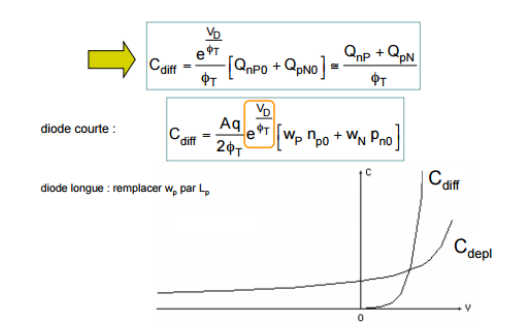
\includegraphics[scale=0.7]{capa}
		\end{solfig}

	
		\item La formule pour la capacité de diffusion est sur la photo du point 2. La capacité de transition vaut $$C_{depl}=\frac{C_{j0}}{(1-V/\phi_T)^m}$$ avec $m=1/2$ pour une jonction abrupte, et $C_{j0}$ qui est un paramètre qui dépend uniquement du modèle de jonction (et non de $V$).
		 La capacité de diffusion est nettement supérieure lorsque la tension vaut 0,7V car elle suit une loi exponentielle.
	\end{enumerate}
	
	
\end{solution}

\section{Exercice (questionnaire B)}
	
	On considère la jonction NP en silicium représentée sur la figure 1 ci-dessous. La zone P ainsi que la zone de déplétion sont protégées de toute illumination par un cache. La zone N n'est par contre pas couverte et soumise à une génération constante G. La structure est suffisamment fine ($h \approx 0$) de sorte que les termes de génération peuvent être considérés constants dans le volume de la zone N. La zone de déplétion est supposée équitablement répartie entre les deux zones N et P, et est de longueur $d$ donnée. On supposera que la génération/recombinaison dans cette zone est constante et donnée par le facteur $U_0$. Une différence de potentiel $V$ est appliquée aux bornes de la diode (entre $x = - x_n$ et $x= x_p$) via des contacts ohmiques. On suppose $N_A$ et $N_D$ connus ainsi que $D_n$, $D_p$, $\tau_n$, $\tau_p$, $T$, $V$, $G$ et $U_0$.
	
	On supposera également que $x_p$ << $L_n$ et $x_n$ >> $L_p$.
	
	\begin{figure}[h!]
		\centering
		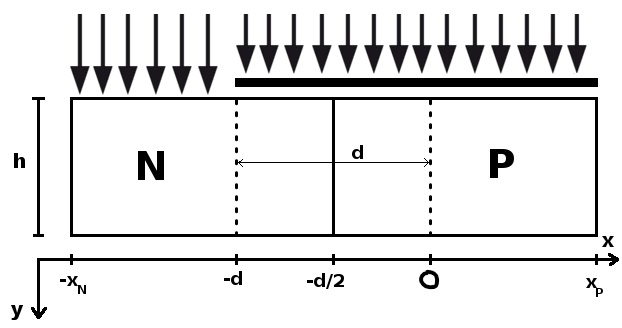
\includegraphics[scale=0.5]{interro}
		\caption{Jonction NP}
		\label{Jonction NP}
	\end{figure}
	
	On vous demande de trouver l'équation de la densité de courant $J$ dans la diode. \\
	
	Énoncez et justifiez clairement toutes les hypothèses simplificatrices que vous utilisez au cours de votre développement. \\
	
	\begin{enumerate}
		\item Déterminez les expressions générales des concentrations en porteurs minoritaires et de la densité de courant dans les deux zones quasi-neutres de la diode à partir des équations de transport.
		\item Donnez les conditions limites nécessaires au calcul de la densité de courant, pour chaque zone et chaque densité de courant en porteurs minoritaires. 
		\item Donnez l'expression de la densité de courant dans la diode en fonction des densités de courant dans chaque zone de la diode et éventuellement des termes de génération/recombinaison.
		\item En développant l'expression obtenue au point précédent, donnez l'expression finale du courant selon les paramètres connus du dispositif.
	\end{enumerate}
	
	Aide - La solution à une équation différentielle du type :
	
	\begin{equation*}
		\frac{\partial f}{\partial x^2} -kf = 0 \hspace{1cm} \text{est donnée par :} \hspace{1cm} f(x) = Ae^{\sqrt{k}x} + Be^{-\sqrt{k}x}
	\end{equation*}
	
	Décrivez qualitativement mais le plus précisément possible : 
	
	\begin{enumerate}
		\setcounter{enumi}{4}
		\item Que se passerait-il si le temps de vie des électrons augmente ? Discutez l'influence de ce paramètre sur vos hypothèses de calcul ainsi que sur l'intensité du courant total.
	\end{enumerate}
	
	\bigskip
	
	\textbf{REMARQUE :} Le formulaire de la partie dispositifs était fourni.

	\begin{solution}
		
		\begin{enumerate}
		\item Dans les zones quasi-neutres, on suppose que le champ électrique est négligeable ($E =0$). On décide de travailler avec les concentrations en porteurs minoritaires car comme
		on le verra par la suite, les relations de Boltzmann peuvent être appliquées pour ces minoritaires. En utilisant les équations pour ces porteurs minoritaires (électrons dans la
		zone P et trous dans la zone N) dans chaque zone quasi-neutre, on obtient:
		$$ \mbox{Zone N: } D_p\frac{\partial^2 p}{\partial x^2}(x)-\frac{p(x)-p_0}{\tau_p}+G=0 \quad (x<-d)$$
		$$ \mbox{Zone P: }  \frac{\partial^2 n}{\partial x^2}(x)=0\quad (x>0)$$
		sous les hypothèses d'une jonction N longue ($x_n >> L_p$), d'une jonction P courte ($x_p << L_n$) et d'un problème stationnaire.
		
		On a donc comme solution des équations dans chacune des zones quasi neutres pour les porteurs minoritaires:
		$$ n(x)=A_n x+B_n \quad (x>0)$$
		$$ p(x)=p_0+A_p e^{\frac{-x}{\sqrt{D_p\tau_p}}}+B_p e^{\frac{x}{\sqrt{D_p\tau_p}}}+\tau_n G \quad (x<-d)$$
		\item De manière à déterminer les différentes constantes du problème, il convient d’imposer
		4 conditions limites en supposant que les relations de Boltzmann se
		vérifient aux limites de la zone de déplétion:
		$$n(x_p)=n_0$$
		$$n(0)=n_0 e^{V/\phi_T}$$
		$$p(-d)=p_0 e^{V/\phi_T}$$
		$$p(-x_n)\neq \infty$$
		On a donc comme
		concentration de porteurs minoritaires dans les zones quasi-neutres:
		$$ n(x)=-n_0 \frac{x}{x_p}(e^{V/\phi_T}-1)+n_0 e^{V/\phi_T} \quad (x>0)$$
		$$ p(x)=p_0+\bigg( p_0(e^{V/\phi_T}-1)-\tau_p G \bigg) e^{\frac{d+x}{\sqrt{D_p\tau_p}}}+\tau_p G \quad (x<-d)$$
		\item Il reste à déterminer le photocourant, on suppose qu'il s'agit uniquement d'un  courant de diffusion. Pour ce faire, on choisit une section quelconque (car le courant est constant le long de la jonction) et
		on additionne les courants dus aux électrons et aux trous:
		$$J(x)=J_n(-d)+J_p(-d)=J_n(0)+J_p(-d)-q\int_{-d}^0 U_0 \:dx= qD_n\frac{\partial n}{\partial x}(0)-qD_p\frac{\partial p}{\partial x}(-d)-qU_0d$$
		puisque le terme de génération $G$ est nul dans la zone de transition.
		
		\item On trouve donc que 
		$$J(x)=-q(e^{V/\phi_T}-1)\bigg(p_0\sqrt{\frac{D_p}{\tau_p}}+\frac{D_n n_0}{x_p} \bigg)+qG\sqrt{D_p\tau_p}-qU_0d$$
		avec $n_0=n_i^2/N_A$ et  $p_0=n_i^2/N_D$ car la concentration en dopant est nettement supérieure à la concentration intrinsèque.
		
		\item Si $\tau_n$ augmente alors la longueur de diffusion $L_n=\sqrt{D_n\tau_n}$ augmente. Cela ne pose pas de soucis dans la zone P car les électrons se recombineront encore moins, l'hypothèse d'une diode courte est donc toujours valable. Par contre, dans la zone de déplétion, la recombinaison diminuera aussi et ainsi, $U_0$ va diminuer. Le courant (en valeur absolue) diminue donc.
		
	\end{enumerate}
		
	\end{solution}
		
	\section{Théorie (questionnaire B)}
	
	$\bullet$ Utilisez des schémas, formules, outils et concepts de base... et limitez le <<bla-bla>> au strict nécessaire.
	
	\begin{enumerate}
		\item Tracez dans un graphe (en échelle linéaire) et expliquez la courbe caractéristique courant-tension de la diode telle que vue dans le cours. Situez les différents régimes de fonctionnement de manière précise. Indiquez des valeurs numériques typiques.
		\item Détaillez l'équation $I-V$ correspondante au niveau physique et ses limites de validité. Définissez les paramètres technologiques et physiques qui influencent le courant.
		\item Discutez les hypothèses sous-jacentes et écarts entre théorie simple et mesures. Représentez les effets non-idéaux sur graphe $log(I)-V$
	\end{enumerate}
	
	\begin{solution}
		
	Solution brève (voir les notes de cours ou les slides pour plus de précision):\\
	
	\begin{enumerate}
		\item La jonction est bloquée si $V<0,7V$ et est passante si $V>0,7V$. 
		\item La relation courant-tension est $$I=I_{sd}(e^{V/\phi_T}-1)+I_{s,rg}(e^{V/(2\phi_T)}-1)$$ avec $I_{sd}$ proportionnel à $n_i^2$ et $I_{s,rg}$ proportionnel à $n_i$. 
		\item En cas de tension élevée, on arrive en forte injection et la résistance série joue un rôle non négligeable. Le courant suit donc une loi en $e^{V/(2\phi_T)}$. De plus, en tension négative, le courant de fuite de génération/recombinaison est nettement supérieur à celui de diffusion (pour une diode en silicium à température ambiante), il ne faut donc pas négliger ce terme lorsqu'on est en régime bloqué. 
	\end{enumerate}
		
		
	\end{solution}
	
\end{document}
